\documentclass[letter,11pt]{article}
\usepackage[spanish, mexico, activeacute]{babel}
\usepackage{amsmath,amsfonts,amssymb}
\usepackage{fancyhdr}
\usepackage{fancyvrb}
\usepackage{xy}
\usepackage{graphicx}
\usepackage{latexsym}
\usepackage{enumerate}
\usepackage{tabularx}
\usepackage{multirow}
\usepackage{multicol}
\usepackage{hyperref}


\usepackage[numbered,framed]{matlab-prettifier}
\lstMakeShortInline"
\lstset{
  style              = Matlab-editor,
  %basicstyle         = \mlttfamily,
  escapechar         = ",
  mlshowsectionrules = true,
}

\setlength{\oddsidemargin}{-0.5cm}
\setlength{\evensidemargin}{0cm}
\setlength{\textwidth}{17.5cm}
\setlength{\textheight}{24cm}
\setlength{\topmargin}{-1.7cm}

\font\bff=cmbx10 at 10truept
\font\lg=cmdunh10 at 10truept
\font\bl=cmss10 at 10truept

\newcommand{\matlab}{{\sc Matlab} }

\newcommand{\header}{\noindent%
{\lg UNIVERSIDAD DE CONCEPCI\'ON}\hfill
\vskip-4truept
\noindent{\bff FACULTAD DE CIENCIAS}\hfill
\vskip-4truept
\noindent{\bff F\'ISICAS Y MATEM\'ATICAS}\hfill
\vskip-4truept
\noindent{\bl DEPARTAMENTO DE INGENIER\'IA MATEM\'ATICA}\hfill
\vskip4truept\hrule\hrule\vskip4truept
\par
}

\newcommand{\respuesta}[1]{
\noindent\makebox[\textwidth][r]{
\fbox{
\begin{minipage}{\textwidth}
\hfill
\vspace{#1}
\end{minipage}
}}}

\title{T1 521230 2018-1}
\begin{document}
\header
\begin{center}
\textbf{\Large TEST 1 C\'ALCULO NUM\'ERICO 521230}\\
\vspace{5mm}
 \begin{tabular}{p{0.6\textwidth}p{0.35\textwidth}}
	\textbf{Nombre:}    &\textbf{Carrera:}\\ \\
	\textbf{Ayudante:} & \textbf{Matr\'icula:}
 \end{tabular}
 \\
 \vspace{0.2cm}
 \begin{tabular}{||p{2cm}|p{2.1cm}||p{2cm}||}
 \hline
 Pregunta 1 &  Pregunta 2   & Total\\
 \hline
 \vspace{1.5cm}\null & &    \\
 \hline
 \end{tabular}
 \end{center}
 
\begin{enumerate}
\item Considere el conjunto de matrices de orden 4
$$
\left\{
\begin{bmatrix}
1/i & 2i^{-2} \\
2i+1 & 3i
\end{bmatrix}
\right\}
_{i=1}^{100}
$$
Mediante un programa de \matlab y usando la funci\'on \texttt{rank()} decida si estas 100 matrices son o no todas invertibles.

Luego decida si este conjunto de matrices es o no linealmente independiente.

Adjunte el programa al correo. 

\textbf{Desarrollo:} 
El programa debe construir y calcular el rango de todas las matrices del conjunto. Si alguno de estos es distinto de $2$, entonces existe una matriz no invertible.
\begin{lstlisting}
clear all; close all; clc;
for i=1:100
	A{i}=[1/i,2*i^(-2);2*i+1,3*i];
    if(rank(A{i})~=2)
    	disp('Las matrices no son todas invertibles');
    end
end
\end{lstlisting}

y luego ensamblar el sistema de ecuaciones de la combinaci\'on lineal nula de estas 100 matrices y ver si tiene \'unica soluci\'on (puede ser calcul\'andola o viendo el rango de la matriz de coeficientes).
\begin{lstlisting}
B=[];
for i=1:100
    B(1,i)=[A{i}(1,1)];
    B(2,i)=[A{i}(1,2)];
    B(3,i)=[A{i}(2,1)];
    B(4,i)=[A{i}(2,2)];
end
if(rank(B)==4)
    disp('Todas las matrices son l.i.')
end
\end{lstlisting}
\item 
Considere el polinomio
$$
p(x)=\frac{1}{8}\left(63x^5-70x^3+15x\right)
$$
en un rutero de \matlab llamado \texttt{polinomio.m}:
\begin{enumerate}
\item Grafique este polinomio en el intervalo $[-1,1]$ con una l\'inea continua negra.
\item Use el m\'etodo de la bisecci\'on para calcular todas las ra\'ices negativas de $p$, con una tolerancia menor que $10^{-4}$.
\item Calcule todas las restantes ra\'ices positivas de $p$ usando el m\'etodo de Newton--Raphson, con una tolerancia menor que $10^{-6}$.
\item Grafique las ra\'ices  positivas del polinomio usando c\'irculos rojos y las negativas usando c\'irculos azules.
\end{enumerate}
Adjunte el programa solicitado y todas las funciones o programas necesarios para su ejecuci\'on.

\textbf{Desarrollo:} Pueden venir anexas dos funciones que implementen los m\'etodos de bisecci\'on y/o de Newton--Raphson, similares a
\begin{lstlisting}
function xr=bisec(f,xa,xb,tol)                                    
while abs(xa-xb)>=tol           	%
    xr=(xa+xb)/2;                   %
    if f(xa)*f(xr)<0                %
        xb=xr;                      %
    else
        xa=xr;                      %
    end
end
\end{lstlisting}

\begin{lstlisting}
function x1=newtonR(f,df,x0,tol)
x1=x0+tol;
while abs(x0-x1)>=tol                          %
  x1=x0-f(x0)/df(x0);                          %
  x0=x1;
end
\end{lstlisting}

El programa \texttt{polinomio.m} debe tener instrucciones similares a
\begin{lstlisting}
clear all; close all; clc;
f=@(x) 1/8*(23*x.^5-70*x.^3+15*x);
df=@(x) 1/8*(23*5*x.^4-70*3*x.^2+15);
x=-1:0.01:1;
plot(x,f(x),'-k');
raicesN=[bisec(f,-0.9,-0.75,10^(-4)),bisec(f,-0.75,-0.25,10^(-4))]; 
	%Raices negativas
raicesP=[newtonR(f,df,0.5,10^(-6)),newtonR(f,df,0.75,10^(-6))]
	%Raices positivas

%%Grafica de las raices pedidas
hold on;
plot(raicesN,f(raicesN),'or',raicesP,f(raicesP),'ob')
\end{lstlisting}

\item Descargue el archivo disponible en
\begin{center}
\url{https://goo.gl/K2fZZZ}
\end{center}
este archivo contiene una matriz que en su primera columna tiene el precio diario, durante los \'ultimos 22 d\'ias, de la acci\'on de \texttt{Cencosud S.A.} y en su segunda columna la cantidad de acciones transadas de esta empresa en cada d\'ia.

En un rutero de \matlab llamado \texttt{acciones.m}
\begin{enumerate}
\item Calcule el promedio de transacciones diarias para estos d\'ias.
\item Grafique el precio diario de la acci\'on de \texttt{Cencosud S.A.} versus el d\'ia.
\item Calcule y grafique el polinomio interpolante del precio diario de acci\'on de \texttt{Cencosud S.A.}

\textquestiondown Qu\'e observa?, es confiable este interpolante para preveer futuros valores de esta acci\'on.

\item Calcule y grafique el spline c\'ubico natural que interpola el precio diario de la acci\'on de \texttt{Cencosud S.A.}

\end{enumerate}
\textbf{Desarrollo:} El programa \texttt{cencosud.m} debe tener instrucciones similares a las siguientes
\begin{lstlisting}
clear all; close all; clc;
load('cencosud.mat');
media=mean(cencosud(:,2));
plot(cencosud(:,1),'+'); hold on;
pol=polyfit(1:22,cencosud(:,1)',21);
xvec=1:0.1:22;
plot(xvec,polyval(pol,xvec))

figure(2)
sp=spline(1:22,cencosud(:,1));
plot(xvec,ppval(sp,xvec),1:22,cencosud(:,1)','+')
\end{lstlisting}
con lo que se tiene que 
\begin{lstlisting}
>> media=mean(cencosud(:,2))

media =

   2.5957e+06
\end{lstlisting}
y se generan gr\'aficas como
\begin{center}
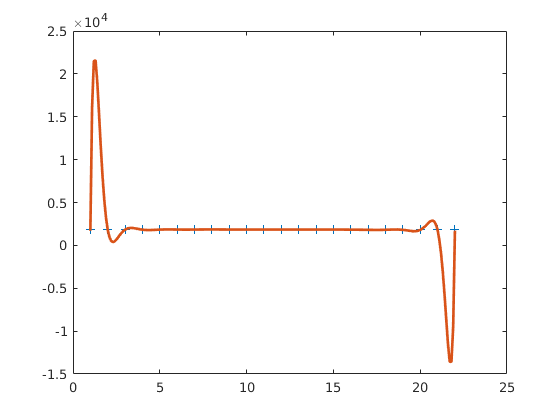
\includegraphics[width=0.8\textwidth]{./cencosud.png}
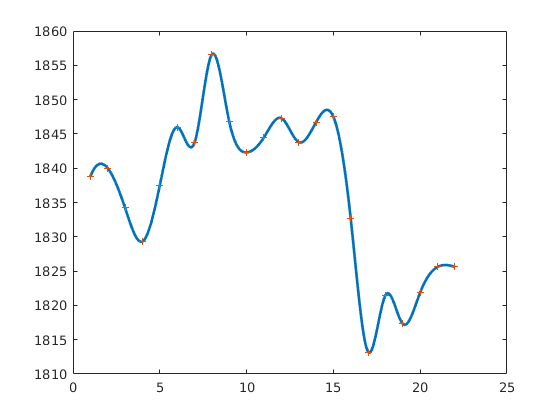
\includegraphics[width=0.8\textwidth]{./cencosud_spline.png}
\end{center}
de donde se responde que, el fen\'omeno de Runge hace poco confiable el interpolante polinomial.
\item 
El modelo de producci\'on de Cobb--Douglas es
$$
P(T,K)=\beta_1 \, T^{\beta_2} \, K^{\beta_3},
$$
donde $P$ es la producci\'on total, $T$ es el trabajo, y $K$ es el capital. En este modelo el par\'ametro $\beta_1$ se interpreta como el factor total de productividad y los par\'ametros $\beta_2$ y $\beta_3$ como las elasticidades del trabajo y capital, respectivamente.

Descargue los datos disponibles en
\begin{center}
\url{https://goo.gl/aJJx4i}
\end{center}
este archivo contiene tres variables \texttt{P}, \texttt{T} y \texttt{K}, que representan respectivamente la producci\'on de salm\'on en Chile medida en toneladas, el valor promedio de un trabajador del salm\'on medido en miles de pesos y el PIB de esta industria medido en millones de d\'olares, durante los \'ultimos 12 meses.

En un rutero de \matlab llamado \texttt{cobbdouglas.m}
\begin{enumerate}
\item Cargue el archivo mencionado anteriormente.
\item Grafique en una misma ventana de figuras, usando \texttt{subplot}, los gr\'aficos de \texttt{P},\texttt{T} y \texttt{K} versus el mes en tras gr\'aficas distintas.
\item A partir de los datos cargados ensamble y resuelva el sistema de ecuaciones lineales que permite calcular, por ajuste de m\'inimos cuadrados, los par\'ametros $\beta_1$, $\beta_2$ y $\beta_3$ de este modelo.

\textbf{Observaci\'on:} Antes de ensamblar las matrices del sistema debe linealizar este modelo. Para esto proponga una transformaci\'on del modelo en el siguiente casillero:

\respuesta{5cm}
\item Escriba a continuaci\'on los valores de los par\'ametros $\beta_1$, $\beta_2$ y $\beta_3$ calculados:

\respuesta{1cm}
\item Calcule la producci\'on, sueldo y PIB promedio de la industria Salmonera durante los \'ultimos 12 meses.
\item Usando los par\'ametros calculados anteriormente, \textquestiondown Cu\'al ser\'ia la producci\'on si se alcanza un PIB promedio pero se duplica el sueldo promedio de los trabajadores?.

\respuesta{1cm}
\end{enumerate}
\textbf{Desarrollo:} 
\begin{enumerate}
\item[a-b)] El programa debe tener instrucciones similares a
\begin{lstlisting}
clear all; close all; clc;
load salmones.mat
subplot(1,3,1);plot(K);
subplot(1,3,2);plot(T);
subplot(1,3,3);plot(P);
\end{lstlisting}
con las cuales se debe hacer un gr\'afico como
\begin{center}
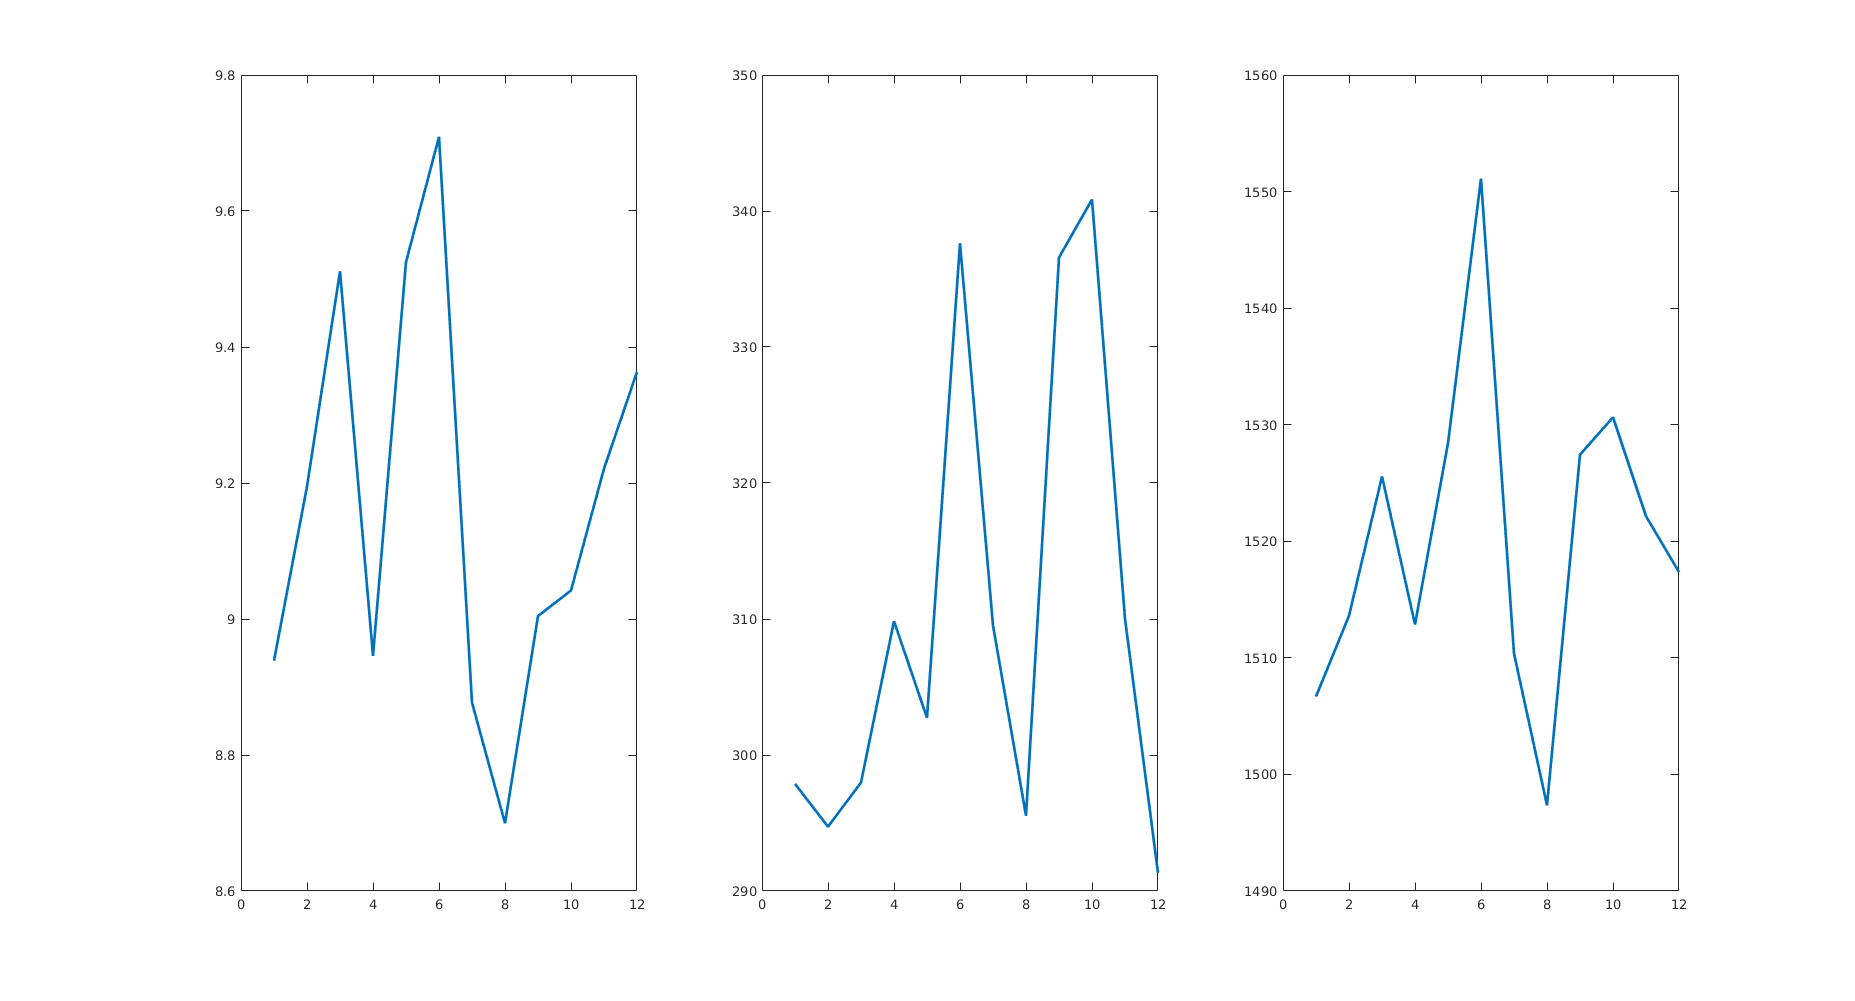
\includegraphics[width=0.8\textwidth]{./cobb-douglas.png}
\end{center}

\item[c)] El modelo se linealiza mediante la funci\'on logaritmo natural, seg\'un
$$
ln(P)=ln(\beta_1)+\beta_2\,T+\beta_3K
$$
de donde se ensambla un sistema matricial similar a
\begin{lstlisting}
>> A=[ones(size(K))',log(T)',log(K)'];
b=log(P)';
coef=A\b

coef =

    6.3099
    0.1000
    0.2000
\end{lstlisting}
\item[d)] De lo anterior sigue que
$$
\beta_1=e^{{6.3099}}=550, \quad \beta_2=0.1,\quad \beta_3=0.2
$$

\item[e)] En el rutero se calculas los promedios de los datos descargados, seg\'un
\begin{lstlisting}
>> kmean=mean(K)
tmean=mean(T)
pmean=mean(P)

kmean =

    9.1693


tmean =

  310.3846


pmean =

   1.5203e+03
\end{lstlisting}
\item Usando los datos anteriores
\begin{lstlisting}
>> nuevaProduccion=exp(coef(1))*(2*tmean)^coef(2)*pmean^coef(3)

nuevaProduccion =

   4.5294e+03
\end{lstlisting}
as\'i en este escenario se producir\'an 4.529 toneladas de salm\'on.
\end{enumerate}


\item Considere el producto interior entre funciones continuas
$$
\langle f,g\rangle =\int_{-\infty}^\infty e^{-x^2}\,f(x)\,g(x) \, dx.
$$
En un rutero de \matlab
\begin{enumerate}
\item Calcule este producto interior entre los polinomios
$$
p(x)=1, \quad q(x)=x, \quad r(x)=x^2,
$$
usando la funci\'on \texttt{quad}.
\item Use las aproximaciones anteriores para decidir, justificadamente, si estos polinomios son o no ortogonales entre ellos.

\respuesta{3cm}

\item Usando las aproximaciones anteriores y el proceso de ortogonalizaci\'on de Gram--Schmidt, ortogonalice, si es necesario, los polinomios $p$, $q$ y $r$.

\respuesta{4cm}

\end{enumerate}

%%%%%%%%% LEONARDO FIGUEROA %%%%%%%%%
\item Sean $\{a_n\}_{n \in \mathbb{N}}$ y $\{c_n\}_{n \in \mathbb{N}}$ las sucesiones definidas por
%
\begin{equation*}
(\forall\,n\in\mathbb{N}) \quad a_n := \frac{n}{2n-1} \quad\text{y}\quad c_n := \frac{n-1}{2n-1}.
\end{equation*}
%
\begin{enumerate}
\item\label{it:JacMat1} Escriba una funci\'on \matlab que reciba un $N \in \mathbb{N}$ y devuelva la matriz $\boldsymbol{A}_N \in \mathbb{R}^{N \times N}$ definida por
%
\begin{equation*}
\boldsymbol{A}_N := \begin{pmatrix}
0 &a_1&&&\\
c_2&\ddots&\ddots&&\\
&\ddots&\ddots&\ddots&\\
&&\ddots &\ddots& a_{N-1}\\\
&&&c_N& 0
\end{pmatrix},
\end{equation*}
%
donde las posiciones sin llenar (arriba de la diagonal $1$ y debajo de la diagonal $-1$) contienen ceros.
\item\label{it:JacMat2} El comando \texttt{eig} de \matlab aplicado a una matriz calcula y devuelve sus autovalores (recolectados en un vector).
Escriba un rutero que grafique en forma de c\'irculos todos los pares ordenados de la forma
%
\begin{equation*}
(\lambda, N)
\end{equation*}
%
donde $\lambda$ es un autovalor de $\boldsymbol{A}_N$, con $N \in \{2, 3, \dotsc, 25\}$.
\end{enumerate}

\textbf{Soluci\'on:} Para la parte \ref{it:JacMat1},
\begin{lstlisting}
function A = matriz(N)
va = (1:N-1)./(2*(1:N-1)-1);
vc = ((2:N)-1)./(2*(2:N)-1);
A = diag(va, 1) + diag(vc, -1);
\end{lstlisting}
Alternativamente,
\begin{lstlisting}
function A = matriz(N)
A = zeros(N);
for n = 1:N-1
    A(n,n+1) = n/(2*n-1);
end
for n = 2:N
    A(n,n-1) = (n-1)/(2*n-1);
end
\end{lstlisting}

Para la parte \ref{it:JacMat2},
\begin{lstlisting}
figure
hold on
for N = 2:25
    lambdas = eig(matriz(N));
    for i = 1:N
        plot(lambdas(i), N, 'o')
    end
end
\end{lstlisting}


\item
Se desea hallar soluciones $\boldsymbol{x} = (x_1, x_2)^\mathtt{t} \in \mathbb{R}^2$ del sistema de ecuaciones no lineales
%
\begin{equation}\label{sistema}
\left\{
\begin{aligned}
x_1^3 - 3 \, x_1 \, x_2^2 & = 1,\\
3 \, x_1^2 \, x_2 - x_2^3 & = 0
\end{aligned}
\right.
\end{equation}
%
mediante el m\'etodo de Newton.

\begin{enumerate}
\item\label{it:f_and_Df} (30\%) Halle una funci\'on vectorial $\boldsymbol{f} \colon \mathbb{R}^2 \to \mathbb{R}^2$ que permita expresar \eqref{sistema} en la forma $\boldsymbol{f}(\boldsymbol{x}) = \boldsymbol{0}$.
Calcule su matriz jacobiana $\boldsymbol{D} \boldsymbol{f} \colon \mathbb{R}^2 \to \mathbb{R}^{2 \times 2}$.
Complete las f\'ormulas de $\boldsymbol{f}$ y $\boldsymbol{D} \boldsymbol{f}$ que aparecen a continuaci\'on.
%
\newcommand{\anchoextra}{\rule{3em}{0pt}}
\begin{equation}\label{f}
\left(\forall\,\boldsymbol{x} = (x_1, x_2)^\mathtt{t} \in \mathbb{R}^2\right) \quad \boldsymbol{f}(\boldsymbol{x}) =
\underbrace{%
\begin{pmatrix}
\anchoextra\phantom{x_1^3 - 3 \, x_1 \, x_2^2 - 1}\anchoextra\\[3ex]
\anchoextra\phantom{3 \, x_1^2 \, x_2 - x_2^3}\anchoextra
\end{pmatrix}}_{\text{Complete aqu\'i}}.
\end{equation}

\begin{equation}\label{Df}
\left(\forall\,\boldsymbol{x} = (x_1, x_2)^\mathtt{t} \in \mathbb{R}^2\right) \quad \boldsymbol{D} \boldsymbol{f}(\boldsymbol{x}) =
\underbrace{%
\begin{pmatrix}
\anchoextra\phantom{3\, x_1^2 - 3\, x_2^2}\anchoextra & \anchoextra\phantom{-6 \, x_1 \, x_2}\anchoextra\\[3ex]
\anchoextra\phantom{6 \, x_1 \, x_2}\anchoextra & \anchoextra\phantom{3\, x_1^2 - 3 \, x_2^2}\anchoextra
\end{pmatrix}}_{\text{Complete aqu\'i}}.
\end{equation}

\item\label{it:it} (30\%) Escriba una funci\'on \matlab que reciba un $\boldsymbol{x}^{(k)} \in \mathbb{R}^2$ y devuelva
%
\begin{equation*}
\boldsymbol{x}^{(k+1)} = \boldsymbol{x}^{(k)} - \boldsymbol{D}\boldsymbol{f}(\boldsymbol{x}^{(k)})^{-1} \boldsymbol{f}(\boldsymbol{x}^{(k)});
\end{equation*}
%
esto es, el iterado de $\boldsymbol{x}^{(k)}$ seg\'un el m\'etodo de Newton para aproximar soluciones del sistema \eqref{sistema}.
\textbf{Sin embargo, no use la funci\'on \texttt{inv}; use \texttt{\textbackslash}.}

\medskip
\noindent ?`C\'omo nombr\'o a su funci\'on?\newline
\noindent{\def\arraystretch{1.5}
\begin{tabularx}{\linewidth}{|p{1.5in}|X|}\hline
nombre funci\'on & \\\hline
\end{tabularx}}

\bigskip

\item\label{it:initial_guesses} (40\%) Escriba un rutero \matlab que
\begin{enumerate}
\item Dada la iteraci\'on inicial $\boldsymbol{x}^{(0)} = \texttt{[0.18; -0.10406]}$ use el programa escrito en la parte \ref{it:it} para calcular la iteraci\'on $\boldsymbol{x}^{(30)}$ del m\'etodo de Newton aplicado al sistema \eqref{sistema} y el valor $\| \boldsymbol{f}(\boldsymbol{x}^{(30)}) \|_2$.
\item Dada la iteraci\'on inicial $\boldsymbol{\tilde x}^{(0)} = \texttt{[0.18; -0.10405]}$ use el programa escrito en la parte \ref{it:it} para calcular la iteraci\'on $\boldsymbol{\tilde x}^{(30)}$ del m\'etodo de Newton aplicado al sistema \eqref{sistema} y el valor $\| \boldsymbol{f}(\boldsymbol{\tilde x}^{(30)}) \|_2$.
\end{enumerate}
%

\medskip
\noindent Complete la siguiente tabla\newline
\noindent{\def\arraystretch{1.5}
\begin{tabularx}{\linewidth}{|p{0.27in}|X|p{0.67in}|X|}\hline
$\boldsymbol{x}^{(30)}$ & \phantom{$\begin{bmatrix} \text{\texttt{-0.50000}} \\ \text{\texttt{0.86603}} \end{bmatrix}$} & $\|\boldsymbol{f}(\boldsymbol{x}^{(30)})\|_2$ & \phantom{\texttt{7.0778e-08}} \\\hline
$\boldsymbol{\tilde x}^{(30)}$ & \phantom{$\begin{bmatrix} \text{\texttt{1.0000e+00}} \\ \text{\texttt{2.7504e-15}} \end{bmatrix}$} & $\|\boldsymbol{f}(\boldsymbol{\tilde x}^{(30)})\|_2$ & \phantom{\texttt{5.1294e-14}} \\\hline
\end{tabularx}}

\medskip
\noindent ?`C\'omo nombr\'o a su rutero?\newline
\noindent{\def\arraystretch{1.5}
\begin{tabularx}{\linewidth}{|p{1in}|X|}\hline
nombre rutero & \\\hline
\end{tabularx}}

\end{enumerate}

\textbf{Desarrollo:} En la parte \ref{it:f_and_Df}, $\boldsymbol{f}(\boldsymbol{x}) = \begin{pmatrix} x_1^3 - 3 \, x_1 \, x_2^2 - 1\\ 3 \, x_1^2 \, x_2 - x_2^3\end{pmatrix}$, $\boldsymbol{D} \boldsymbol{f}(\boldsymbol{x}) = \begin{pmatrix} 3\, x_1^2 - 3\, x_2^2 & -6 \, x_1 \, x_2 \\ 6 \, x_1 \, x_2 & 3\, x_1^2 - 3 \, x_2^2 \end{pmatrix}$.

Un programa como el pedido en la parte \ref{it:it} es:
\begin{lstlisting}
function nuevox = iteracionNewtonSistemaCubico(x)
f = [
    x(1)^3-3*x(1)*x(2)^2-1;
    3*x(1)^2*x(2)-x(2)^3
    ];
Df = [
    3*x(1)^2-3*x(2)^2 -6*x(1)*x(2);
    6*x(1)*x(2) 3*x(1)^2-3*x(2)^2
    ];
nuevox = x - Df\f;
\end{lstlisting}

Un rutero como el pedido en la parte \ref{it:initial_guesses} es:
\begin{lstlisting}
x = [0.18; -0.10406];
for i = 1:30
    x = iteracionNewtonSistemaCubico(x);
end
x
fx = [
    x(1)^3-3*x(1)*x(2)^2-1;
    3*x(1)^2*x(2)-x(2)^3
    ];
normfx = norm(fx)

xtilde = [0.18; -0.10405];
for i = 1:30
    xtilde = iteracionNewtonSistemaCubico(xtilde);
end
xtilde
fxtilde = [
    xtilde(1)^3-3*xtilde(1)*xtilde(2)^2-1;
    3*xtilde(1)^2*xtilde(2)-xtilde(2)^3
    ];
normfxtilde = norm(fxtilde)
\end{lstlisting}

En mi sistema (que en vez de \matlab tiene \textsc{Octave}; podr\'ia ser que en \matlab los resultados sean ligeramente distintos; tambi\'en cabe esperar resultados ligeramente distintos si se elige un $\boldsymbol{f}$ equivalente pero distinto) obtengo:
\begin{gather*}
\boldsymbol{x}^{(30)} = \begin{bmatrix} \text{\texttt{-0.50000}} \\ \text{\texttt{0.86603}} \end{bmatrix}, \quad \|\boldsymbol{f}(\boldsymbol{x}^{(30)})\|_2 = \text{\texttt{7.0778e-08}},\\
\boldsymbol{\tilde x}^{(30)} = \begin{bmatrix} \text{\texttt{1.0000e+00}} \\ \text{\texttt{2.7504e-15}} \end{bmatrix}, \quad \|\boldsymbol{f}(\boldsymbol{\tilde x}^{(30)})\|_2 = \text{\texttt{5.1294e-14}}.
\end{gather*}

\item 
Se desea aproximar la funci\'on $f$ definida por $f(x) = \exp(-x)$ en el intervalo $[-1,1]$ por polinomios.
Construiremos tres alternativas.

\begin{enumerate}
\item\label{it:three_polynomials_N} (70\%) Escriba una funci\'on \matlab que reciba un grado $N \in \mathbb{N}_0 = \{0, 1, 2, \dotsc \}$ y
devuelva los siguientes tres polinomios:
\begin{itemize}
\item El polinomio $p$ que resulta de interpolar la funci\'on $f$ en $N+1$ puntos equiespaciados en $[-1,1]$ incluyendo los extremos; esto es, en
%
\begin{equation*}
\text{\texttt{linspace(-1, 1, N+1)}}
\end{equation*}
%
\item El polinomio $q$ que resulta de interpolar la funci\'on $f$ en los $N+1$ puntos de cuadratura de Gauss--Lobatto--Chebyshev, los que se pueden expresar como
%
\begin{equation*}
\text{\texttt{cos(linspace(0, pi, N+1))}}
\end{equation*}
%
\item El polinomio $r$ que resulta de truncar la serie de Taylor para la funci\'on $f$ centrada en $0$ hasta el t\'ermino de grado $N$; esto es,
%
\begin{equation*}
r(x) = \sum_{n=0}^N \frac{(-1)^n}{n!} x^n.
\end{equation*}
%
\end{itemize}
%
Cada uno de estos polinomios debe ser entregado por la funci\'on en el formato que usa la funci\'on de \matlab \texttt{polyval}; as\'i, por ejemplo, cuando $N = 5$ el polinomio $r$ debe quedar representado por el vector de coeficientes
%
\begin{equation*}
\text{\texttt{[-1/120  1/24  -1/6  1/2  -1  1]}}
\end{equation*}
%
en ese orden. Recuerde tambien que en \matlab la funci\'on exponencial se llama \texttt{exp} y la funci\'on factorial se llama \texttt{factorial}.

\medskip
\noindent ?`C\'omo nombr\'o a su funci\'on?\newline
\noindent{\def\arraystretch{1.5}
\begin{tabularx}{\linewidth}{|p{1.1in}|X|}\hline
nombre funci\'on & \\\hline
\end{tabularx}}

\bigskip

\item\label{it:three_polynomials_13} (30\%) Escriba un rutero \matlab que
\begin{itemize}
\item llame al programa de la parte anterior para obtener $p$, $q$ y $r$ cuando $N = 13$ y
\item dibuje $f(x) - p(x)$, $f(x) - q(x)$ y $f(x) - r(x)$ con $x \in [-1, 1]$ en un mismo gr\'afico.
\end{itemize}

\medskip
\noindent ?`C\'omo nombr\'o a su rutero?\newline
\noindent{\def\arraystretch{1.5}
\begin{tabularx}{\linewidth}{|p{1in}|X|}\hline 
nombre rutero & \\\hline
\end{tabularx}}
\end{enumerate}

\textbf{Desarrollo:} Una funci\'on apropiada para la parte \ref{it:three_polynomials_N} es
\begin{lstlisting}
function [p, q, r] = trespolis(N)
xp = linspace(-1, 1, N+1);
p = polyfit(xp, exp(-xp), N);
xq = cos(linspace(0, pi, N+1));
q = polyfit(xq, exp(-xq), N);
r = [];
for n = N:-1:0
    nuevocoef = (-1)^n/factorial(n);
    r = [r nuevocoef];
end
\end{lstlisting}

Un rutero apropiado para la parte \ref{it:three_polynomials_13} es
\begin{lstlisting}
[p, q, r] = trespolis(13);
xx = linspace(-1, 1, 100);
% una alternativa a esta manera de dibujar tres curvas juntas es usar
% 'hold on' y luego dibujarlas por separado
plot(xx, exp(-xx) - polyval(p, xx), '-', ...
     xx, exp(-xx) - polyval(q, xx), '-', ...
     xx, exp(-xx) - polyval(r, xx), '-')
\end{lstlisting}


\item
Se desea ajustar los par\'ametros $c_1, \dotsc, c_4$ del modelo
%
\begin{equation*}
f(\theta) = c_1 + c_2 \frac{\sen(2\theta)}{\sen(\theta)} + c_3 \frac{\sen(3\theta)}{\sen(\theta)} + c_4 \frac{\sen(4\theta)}{\sen(\theta)}
\end{equation*}
%
a los puntos $(\theta_i, f_i)$, $i \in \{1, \dotsc, 8\}$, descritos en la siguiente tabla:
%
\begin{center}
\begin{tabular}{c|cccccccc}
$\theta_i$ & 0.36 & 1.46 & 1.53 & 1.81 & 2.24 & 2.46 & 2.72 & 2.84\\\hline
$f_i$ & 0.48 & 0.21 & 0.08 & -0.44 & -0.97 & -0.97 & -0.63 & -0.31
\end{tabular}
\end{center}

Escriba un rutero \matlab que realice el ajuste y grafique conjuntamente la curva ajustada en el intervalo $\theta \in [0,\pi]$ y los ocho pares ordenados de la tabla (recuerde que en \matlab la funci\'on seno se llama \texttt{sin}).

Complete la siguiente tabla:

\noindent{\def\arraystretch{1.5}%
\begin{tabularx}{\linewidth}{|p{1em}|X|p{1em}|X|p{1em}|X|p{1em}|X|}\hline
$c_1$ & & $c_2$ & & $c_3$ & & $c_4$ & \\\hline
\end{tabularx}%
}

\medskip
\noindent ?`C\'omo nombr\'o a su rutero?\newline
\noindent{\def\arraystretch{1.5}
\begin{tabularx}{\linewidth}{|p{1in}|X|}\hline 
nombre rutero & \\\hline
\end{tabularx}}

\textbf{Desarrollo:} Un rutero que realiza las tareas solicitadas es:
\begin{lstlisting}
t = [0.36 1.46 1.53 1.81 2.24 2.46 2.72 2.84]';
f = [0.48 0.21 0.08 -0.44 -0.97 -0.97 -0.63 -0.31]';
A = [ones(size(t)) sin(2*t)./sin(t) sin(3*t)./sin(t) sin(4*t)./sin(t)];
c = A\f
tt = linspace(0,pi,512);
ff = c(1) + c(2)*sin(2*tt)./sin(tt) + c(3)*sin(3*tt)./sin(tt) + c(4)*sin(4*tt)./sin(tt);
plot(tt, ff, '-', t, f, 'o')
\end{lstlisting}

En \textsc{Octave} obtuve \texttt{c = [-0.0045619; 0.6630383; -0.0011977; -0.2696056]}.

A alguien podría ocurr\'irsele multiplicar el modelo por $\sen(\theta)$ y aplicar m\'inimos cuadrados a ese modelo modificado.
Eso tambi\'en es admisible.
En ese caso los par\'ametros ajustados son parecidos pero distintos: \texttt{c = [-0.021768; 0.628855; -0.019332; -0.229573]}.


%%%%%%%%% MAURICIO VEGA %%%%%%%%%
%% Matlab
\item Considere la sucesi\'on de Fibonacci, dada por:
$$
f_{n+1}=f_n+f_{n-1}, \qquad n=1,2,3,\ldots,
$$
con $f_0=0$ y $f_1=1$. 
\begin{enumerate}
\item Escriba una funci\'on en \matlab que, dado un valor de entrada $n\in \mathbb{N}$, devuelva como salidas, el valor de $f_{n+1}$, el cuociente $f_{n+1}/f_n$ y el valor $|f_{n+1}/f_n-\varphi|$, donde $\varphi=(1+\sqrt{5})/2$ es el n\'umero dorado.
\item Escriba un rutero en \matlab que llame a la funci\'on anterior y muestre sus salidas, para cada valor $n\in \{1, 10, 100, 1000\}$.
\item >Qu\'e relaci\'on existe entre el cuociente $f_{n+1}/f_n$ y el n\'umero dorado $\varphi$? Justifique en base a los resultados obtenidos en el siguiente casillero.\bigskip

\respuesta{2cm}
\end{enumerate}
\textbf{Desarrollo:}  Cada programa viene dado por:
\begin{lstlisting}
function [fnp1,cuociente,err] = fibonacci(n)
fnm1 = 0;
fn = 1;
for i=1:n
    fnp1 = fn + fnm1;
    cuociente = fnp1 / fn;
    fnm1 = fn;
    fn = fnp1;
end
phi = (1 + sqrt(5)) / 2; 
err = abs(cuociente - phi);
\end{lstlisting}

\begin{lstlisting}
N = [1, 10, 100, 1000];
for i = 0:3;
    [fn, cuociente, err] = fibonacci(N(i+1))
end
\end{lstlisting}

La relaci\'on entre el cuociente $f_{n+1}/f_n$ y el n\'umero dorado $\varphi$ est\'a dada por $\displaystyle \lim_{n\to \infty}\dfrac{f_{n+1}}{f_n}=\varphi$. Esto puede ser notado en el decrecimiento de los errores $|f_{n+1}/f_n-\varphi|$ a medida que aumenta $n$

\hfill\fbox{30 puntos}.

%%%%%% Ec. No Lineales.
\item Considere la funci\'on $f(x,y)=\cos(x)+\sen(y)$. Escriba un rutero en \matlab que encuentre un punto cr\'itico de $f$, cercano al punto $(x_0,y_0)=(4,4)$, mediante el m\'etodo de Newton, con un error menor a $10^{-9}$. Su programa debe mostrar la soluci\'on obtenida y el n\'umero de iteraciones que ejecut\'o.

\textbf{Desarrollo:} Considerando que debemos resolver la ecuaci\'on vectorial $\nabla f = \boldsymbol{\theta}$,  el programa est\'a dado por:

\begin{lstlisting}
tol = 10^(-9);
g = inline('[-sin(x);cos(y)]','x','y');
Dg = inline('[-cos(x) 0 ; 0 -sin(y)]','x','y');
x0 = [4;4];
difer = 10*tol;
iter = 0;
while difer >tol
    x1 = x0 - inv(Dg(x0(1),x0(2)))*g(x0(1),x0(2));
    difer = norm(x0 - x1);
    x0 = x1;
    iter = iter + 1;
end
x1
iter
\end{lstlisting}

%%%%%% Interpolacion
\item La interpolaci\'on polinomial de Newton consiste en utilizar la base de polinomios de Newton, dada por: $\{1, x-x_0, (x-x_0)(x-x_1),\ldots,(x-x_0)(x-x_1)\cdots(x-x_{n-1})\}$, para interpolar los puntos $(x_0,y_0)$,\ldots, $(x_n,y_n)$. As\'i, el polinomio que interpola estos puntos est\'a dado por:
$$
p(x)=\alpha_0+\alpha_1(x-x_0)+\alpha_2(x-x_0)(x-x_1)+\cdots+\alpha_n(x-x_0)(x-x_1)\cdots(x-x_n),
$$
donde los coeficientes $\alpha_0,\alpha_1,\ldots,\alpha_n$ se obtienen al resolver el sistema $\boldsymbol{A\alpha}=\boldsymbol{y}$, que se obtiene al evaluar:
$$
p(x_i)=y_i,\qquad \forall\,i=0,\ldots,n.
$$
Escriba un rutero en \matlab que realice las siguientes tareas:
\begin{enumerate}
\item Construya la matriz $\boldsymbol{A}$ y el vector $\boldsymbol{y}$ mencionados anteriormente, considerando los puntos $x_i=-5,-4,\ldots,4,5$ e $y_i=1/(1+x_i^2)$.
\item Resuelva el sistema $\boldsymbol{A\alpha}=\boldsymbol{y}$ y muestre los coeficientes $a_0,\ldots, a_n$ del polinomio de interpolaci\'on de Newton. 
\item Grafique en un mismo gr\'afico la funci\'on $f(x)=1/(1+x^2)$ (l\'inea continua), el polinomio de interpolaci\'on de Newton $p(x)$ (l\'inea discontinua) y los puntos a interpolar (c\'irculos).
\end{enumerate}
>Qu\'e fen\'omeno observa en la gr\'afica? >Se puede evitar este fen\'omeno utilizando el polinomio de interpolaci\'on de Lagrange? Justifique su respuesta. \bigskip

\respuesta{3cm}
\medskip

\textbf{Desarrollo:} El rutero est\'a dado por:

\begin{lstlisting}
x = [-5:5]';
y = 1./(1+x.^2);
n = length(x);
A = ones(n,1);
aux = x - x(1);
for i=2:n
    A = [A aux];
    aux = aux.*(x - x(i));
end
alpha = A\y
xx = [-5:0.01:5]';
yy = 1./(1+xx.^2);
nn = length(xx);
aux = ones(nn,1);
pp = zeros(nn,1);
for i=1:n;
    pp = pp + alpha(i)*aux;
    aux = aux.*(xx-x(i));
end
plot(xx,yy,'-',xx,pp,'--',x,y,'o')
legend('y=1/(1+x^2)','Int. Newton', 'Puntos')
\end{lstlisting}
mientras que la gr\'afica est\'a dada por:

\centerline{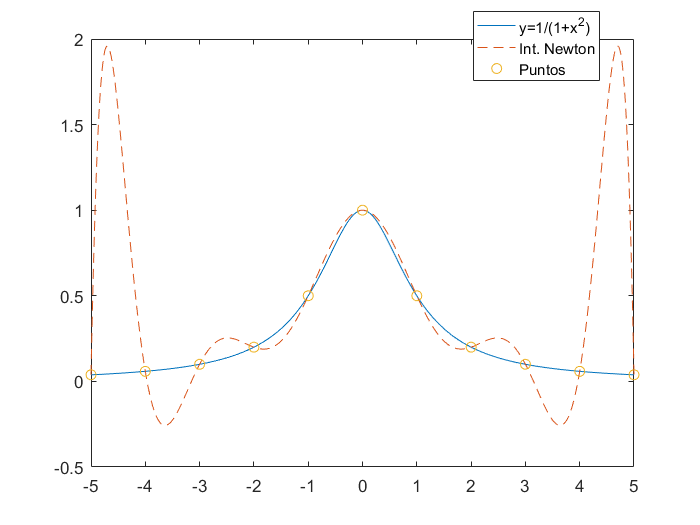
\includegraphics[width=0.6\textwidth]{inter_newton.png}}

El polinomio de interpolaci\'on de Newton presenta el fen\'omeno de Runge, el cual no puede ser evitado por la interpolaci\'on de Lagrange, debido a que el polinomio de interpolaci\'on es \'unico, independiente de la base utilizada para calcularlo (can\'onica, Lagrange o Newton).

%%%%%% Minimos Cuadrados
\item Los resultados de cierto experimento relacionan las variables $x$ e $y$, mediante el modelo:
$$
y=\beta x^{\alpha x}.
$$
Estos resultados se muestran en la siguiente tabla:
\begin{center}
\begin{tabular}{c|ccccc}
$x$ & 1 & 1.5 & 2 & 3 & 4\\
\hline
$y$ & 85 & 60 & 15 & 3 & 1
\end{tabular}
\end{center}
Escriba un rutero en \matlab que realice las siguientes tareas:
\begin{enumerate}
\item Calcule y muestre los par\'ametros $\alpha$ y $\beta$ que ajustan el modelo a los datos de la tabla en el sentido de los m\'inimos cuadrados.
\item En un mismo gr\'afico dibuje los puntos de la tabla (c\'irculos) y el modelo ajustado anteriormente (linea continua).
\item Estime y muestre el valor de $y$ cuando $x=5$.
\end{enumerate}

\textbf{Desarrollo:} El rutero est\'a dado por:

\begin{lstlisting}
x=[1 1.5 2 3 4]';
y=[85 60 15 3 1]';
A = [ones(5,1) x.*log(x)];
B = log(y);
X = A\B
alpha = X(2);
beta = exp(X(1));
xx = 1:0.01:4;
yy = beta*xx.^(alpha*xx);
plot(x,y,'o',xx,yy,'-')
legend('Datos','Modelo')
x5=5;
y5 = beta*x5.^(alpha*x5)
\end{lstlisting}
mientras que el gr\'afico est\'a dado por:

\centerline{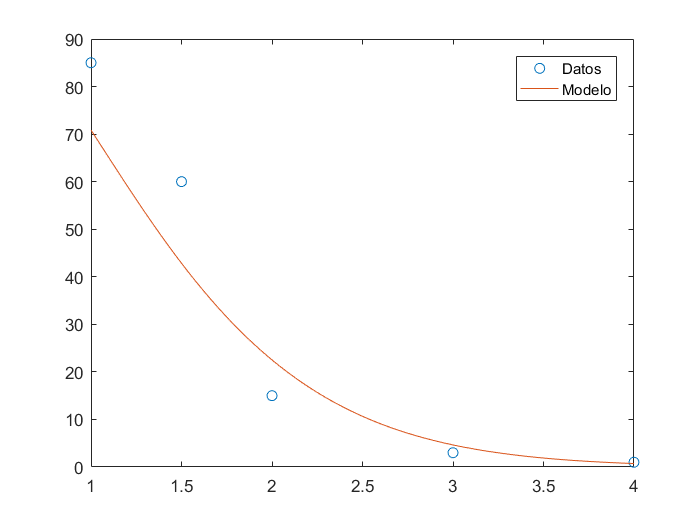
\includegraphics[width=0.6\textwidth]{mincuad.png}}
\end{enumerate}

\end{document}
